\chapter{Konzeption}
\label{cha:konzeption}

In diesem Kapitel werden die Anforderungen an den Chatbot und ein Konzept für die Implementierung erarbeitet.  Dafür werden Ansichten und Methoden aus dem Bereich \textit{Usability Engineering} verwendet. Usability wird auch als Gebrauchstauglichkeit bezeichnet und definiert sich wie folgt: 

\begin{quote}
    Das Ausmaß, in dem ein Produkt durch bestimmte Benutzer in einem bestimmten Nutzungskontext dazu genutzt werden kann, bestimmte Ziele effektiv, effizient und zufriedenstellend zu erreichen \cite[S. 11]{richter_usability_2016}.
\end{quote}

Der \textit{Nutzungskontext} umfasst dabei die Benutzer, deren Aufgaben, soziale und physische Umgebung sowie die aufgewendeten Ressourcen. Die \textit{Effektivität} misst dabei die Vollständigkeit und Genauigkeit der Zielerreichung. Das Kriterium \textit{Effizienz} bezeichnet den Aufwand und die Ressourcen zur Zielerreichung. Die \textit{Zufriedenstellung} gibt Auskunft über die Freiheit von Beeinträchtigungen und positive Einstellung des Benutzers gegenüber dem System. 

Die Definition von Usability impliziert dabei jedoch immer eine sehr funktionsbezogene Betrachtungsweise. Um auch Aspekte wie Emotionen, Ästhetik und Wahrnehmungen zu betrachten, kann das Konzept der \textit{\ac{UX}} angewendet werden. Die \acl{UX} erweitert die Usability und definiert sich wie folgt:

\begin{quote}
   Wahrnehmungen und Reaktionen einer Person, die aus der tatsächlichen und/oder der erwarteten Benutzung eines Produktes, eines Systems oder einer Dienstleistung resultieren \cite[S. 14]{gast_user_2018}.
\end{quote}

\ac{UX} umfasst demnach auch Effekte auf den Nutzer, die ein System bereits vor oder auch nach seiner Verwendung hat. Diese Empfindungen haben wiederum Einfluss auf den nachfolgenden Aspekt (\textit{„Nach der Nutzung ist vor der Nutzung“}).
Die Usability bleibt dennoch ein wichtiger Faktor und Teil der \acl{UX}. Aufgrund der umfassenderen Betrachtungsweise wird der Begriff \ac{UX} immer öfter auch anstelle der Bezeichnung \textit{Usability} verwendet. Abbildung \ref{fig:usability-user-experience} erläutert die beiden Begriffe anhand einer grafischen Darstellung.
\newline

\begin{figure}[htb]
    \centering
    \includegraphics[width=0.8\textwidth]{bilder/usability-user-experience_v2.png}
    \caption{Usability und \acl{UX}}
    \label{fig:usability-user-experience}
\end{figure}

Sowohl Usability als auch User Experience stellen einen wichtigen Faktor in der Softwareentwicklung dar. Gerade im Bereich der \aclp{CUI} ist die Anwendung dieser Konzepte und Methodiken äußerst wichtig. Nachdem der Benutzer beim \ac{CUI} auf natürliche Art und Weise mit dem System interagiert, müssen Formulierungen und Ausdrucksweisen fehlerfrei erkannt und interpretiert werden. Zudem müssen auch eventuelle Rückfragen, Statusmeldungen oder Antworten korrekt und ohne Spielraum für Missinterpretationen formuliert werden. 

Ein weiterer wichtiger Aspekt in diesem Zusammenhang ist das \textit{\ac{UCD}}, im Deutschen oft als \textit{menschzentrierter Gestaltungsprozess} übersetzt. Diese nutzerzentrierte Gestaltung zielt darauf ab, interaktive Produkte so zu gestalten, dass sie über eine hohe Gebrauchstauglichkeit verfügen. Der Begriff beschreibt Gestaltungsprozesse, die den zukünftigen Benutzer mit seinen Aufgaben, Zielen und Eigenschaften ins Zentrum des Entwicklungsprozesses stellen. Dabei spielt die frühe Fokussierung auf den Nutzer und dessen Anforderungen eine entscheidende Rolle. Der Prozess sieht außerdem Iterationen vor, sobald Evaluierungsergebnisse Bedarf dafür aufzeigen. \cite[S. 67-68]{tryfonas_human_2016} 

Diese Vorgehensweise hat sich in den letzten Jahren bei der Entwicklung von Mobile- und Webapplikationen bewährt. Die grundlegenden Nutzeranforderungen ändern sich nicht durch einen Wechsel des Interfaces von \ac{GUI} zu \ac{CUI}. Es muss jedoch verstanden werden, welche Methoden und Techniken in diesem Zusammenhang sinnvoll sind und verwendet werden sollten. Werden diese Aspekte bei der Entwicklung eines Chatbots angewendet, so können auch hier wertvolle Daten gesammelt werden, woraus dann hochwertige \aclp{UI} entstehen. \cite{chandra_how_2018} 

Die Inhalte des \textit{\acl{UCD}} sind in der \textit{ISO 9241-210} festgehalten und können anhand von Abbildung \ref{fig:user-centered-design} grafisch dargestellt werden.
\newline

\begin{figure}[htb]
    \centering
    \includegraphics[width=1.0\textwidth]{bilder/user-centered-design.png}
    \caption{\acl{UCD} - Menschzentrierter Gestaltungsprozess \cite{geis_neue_2010}}
    \label{fig:user-centered-design}
\end{figure}

Um all diese Ziele zu erreichen, werden zunächst Überlegungen hinsichtlich des Requirements Engineering angestellt. Dazu können verschiedene Techniken aus dem Bereich des Usability- und Requirements Engineering eingesetzt werden. Mit Hilfe einer prototypischen Umsetzung können diese Überlegungen anschließend überprüft und evaluiert werden.

\section{Requirements Engineering}
\label{sec:requirements-engineering}

Requirements Engineering befasst sich damit, die Bedürfnisse der Benutzer, Auftraggeber
und weiterer Interessengruppen, im Allgemeinen auch als Stakeholder bezeichnet, hinreichend aufzuarbeiten \cite[S. 23]{richter_usability_2016}. Darauf basierend können dann Rückschlüsse auf die Rahmenbedingungen, Qualitätsanforderungen sowie vorgesehene Funktionen und Systemverhalten geschlossen werden. 

\subsection{Fragebogen}
\label{subsec:fragebogen}

Um einen groben Überblick über die Thematik zu erhalten, sollen zunächst das Verhalten und die Präferenzen bei der Raumbuchung im Office der \adorsys\ erfasst werden. Um eine mögliche Voreingenommenheit gegenüber Chatbots zu vermeiden, wird der Hintergrund und das explizite Thema der Masterarbeit in diesem Zusammenhang nicht erwähnt. Die Zielgruppe sind dabei alle Mitarbeiter der \adorsys\ unabhängig davon, wie oft diese in der Regel einen Raum buchen. 

Um möglichst alle relevanten Informationen einzufangen, soll dazu ein Online-Frage\-bogen erstellt werden. Mit dessen Hilfe lassen sich quantitative Daten sammeln und direkt elektronisch auswerten. Zur Erstellung und Durchführung des Fragebogens werden im Folgenden die Anwendungen \textit{Survey Monkey}, \textit{Typeform} und \textit{Google Forms} genauer betrachtet. Dazu wird, wenn es unterschiedliche Varianten gibt, jeweils die kostenlose Basisvariante der Anwendungen untersucht. Die kostenlosen Varianten der Anwendungen werden verwendet, um möglichst keine Mehrkosten zu generieren sowie den Aufwand und die damit verbundenen Verzögerungen minimal zu halten. Die Anforderungen resultieren aus den Rahmenbedingungen des zuvor erstellten Fragebogens. So besteht dieser aus 18 Fragen, bei denen es sich hauptsächlich um Basis-Fragetypen wie Multiple-Choice, Textfelder oder linearen Skalen handelt. Relevant ist dabei auch die Anonymisierung der Daten, um möglichst ehrliche und ungefilterte Antworten zu erhalten. Das Unterbinden einer Mehrfachteilnahme ist ebenso wünschenswert. 

Der vollständige Fragebogen ist aus Gründen der besseren Lesbarkeit im Anhang \ref{sec:anhang-fragebogen} zu finden. 
Tabelle \ref{tab:umfrage-toolauswahl} zeigt eine Übersicht der Anforderungen und betrachteten Anwendungen. Erfüllte Anforderungen sind dabei mit einem \textit{grünen Haken}, nicht erfüllte mit einem \textit{roten Kreuz} versehen. Ein \textit{gelbes Warndreieck} sagt aus, dass die Anforderung nur unter einer bestimmten Bedingung erfüllt werden kann. Die Inhalte der Tabelle stützen sich auf die Informationen aus \cite{surveymonkey_surveymonkey_2018}, \cite{typeform_plans_2018} und \cite{google_forms_google_2018}.
\newline

\begin{table}[!htb]
\centering
 \begin{tabular}{ | m{5cm} || C{2cm}| C{2cm} | C{2cm} |} 
 \hline
 Anforderungen & Survey Monkey & Typeform & Google Forms 
 \\
 \hhline{=::===}
 18 Fragen & \xmark & \xmark & \cmark\\ 
 \hline Basis-Fragetypen & \cmark & \cmark & \cmark \\
 \hline Anonymisierung & \cmark & \cmark & \cmark\\ 
 \hline Mehrfachteilnahme unterbinden & \cmark & \danger & \cmark\\ 
 \hline
\end{tabular}
\caption{Auswahl einer Anwendung für den Fragebogen}
\label{tab:umfrage-toolauswahl}
\end{table}

Die beiden Anwendungen Survey Monkey und Typeform ermöglichen in der Basisvariante nur maximal zehn Fragen. Bei Google Forms gibt es eine solche Beschränkung dagegen nicht. Die für den Fragebogen relevanten Basis-Fragetypen wie Multiple-Choice, Textfelder oder lineare Skalen unterstützen dagegen alle Anwendungen. Gleiches gilt für die Möglichkeit, die erfassten Daten zu anonymisieren. Die Unterbindung einer Mehrfachteilnahme ist mit Typeform nur über Umwege möglich, wird von Survey Monkey und Google Forms dagegen standardmäßig unterstützt. Aufgrund der erläuterten Kriterien fällt die Wahl der Anwendung auf Google Forms. Die Anwendung unterstützt alle Anforderungen und kann ohne zusätzliche Kosten genutzt werden. 

Im Folgenden werden einige markante Ergebnisse aus dem Fragebogen herausgegriffen und genauer betrachtet. Die Fragen sind dabei oft nach Schlagwörtern wie \textit{gewöhnlich} oder \textit{in der Regel} gestellt und müssen daher mit Vorsicht betrachtet werden, um keine falschen Rückschlüsse auf die Ergebnisse zu ziehen. 

Knapp die Hälfte der Befragten buchen täglich oder alle zwei bis drei Tage einen Raum. Dabei ist erwähnenswert, dass sich der Fragebogen auf die Raumbuchung im Office der \adorsys\ bezieht und einige der Befragten durch Ihre Tätigkeit bei Kunden und in Projekten oft außerhalb des Büros arbeiten. Daraus lässt sich schließen, dass das Buchen von Räumen bei vielen Mitarbeitern ein fester Bestandteil des Arbeitsalltags ist. 

Über 60\,\% der Buchungen werden dabei mindestens einen Tag im Voraus getätigt, mit knapp 2\,\% gibt es vergleichsweise wenige Buchungen über Wochen oder Monate im Voraus. Erklären lässt sich dies dadurch, dass weit im Voraus geplante Termine oft einen Workshop- oder Schulungs-Charakter haben, über mehrere Stunden gehen und eine größere Anzahl an Teilnehmern besitzen. Diese müssen entsprechend frühzeitig geplant werden, kommen aber vergleichsweise selten vor. 

Erwähnenswert ist außerdem das Ergebnis auf die Frage nach der gewöhnlichen Besprechungsdauer. Über 90\,\% der Teilnehmer geben an, dass ihre Besprechungen in der Regel weniger als zwei Stunden dauern. Dies ist möglicherweise auf die Vielzahl an relativ häufigen und gleichermaßen kürzeren Termine wie beispielsweise Code-Reviews, Team-Meetings aber auch Vorstellungs- oder Mitarbeitergesprächen zurückzuführen. 

Einige Fragen beziehen sich auf das \textit{E-Paper Display} am Eingang der Besprechungsräume, welches den aktuellen Status des Raumes sowie das nächste anstehende Meeting anzeigt. Außerdem bietet es durch Bedienung die Möglichkeit, den Belegungsplan des Raumes einzusehen und den Raum direkt oder zu einem späteren Zeitpunkt zu reservieren. Nach den Ergebnissen aus dem Fragebogen nutzen etwa zwei Drittel das E-Paper Display, wenn sie sofort einen Raum benötigen. Um einen Raum zu einem späteren Zeitpunkt zu verwenden, nutzen es dagegen nur knapp 8\,\%. Als Grund hierfür könnte die Bedienung eine Rolle spielen. Wenn sofort ein freier Raum benötigt wird, zeigt das Display den Status des Raumes an und bietet die Möglichkeit, den Raum über einen Klick zu reservieren. Für eine Reservierung zu einem späteren Zeitpunkt ist eine aufwendigere Bedienung des E-Paper Displays nötig. 

Mehr als die Hälfte der Teilnehmer finden eine Bestätigung der Raumbuchung sinnvoll. Als häufigste Gründe dafür werden das Vermeiden von Leerbuchungen und eine gesteigerte Konsistenz von Buchung zum tatsächlichen Status genannt. Auf der Gegenseite stehen Bedenken in Form von Vergessen der Bestätigung sowie Mehrarbeit und zusätzlicher Aufwand bei der Buchung. 

Auf die Frage nach bevorzugten Räumen bei der Buchung gibt es relativ eindeutige Ergebnisse. Knapp 60\,\% der Befragten nannten in diesem Zusammenhang die Räume R1, R2 und R4. Häufig genannte Gründe hierfür sind die angenehme Raumgröße für bis zu acht Personen und die Helligkeit des Raumes durch die großen Fenster (Tageslicht). Den Raum R3 bevorzugen nur etwa 28\,\% der Teilnehmer und führen dies meist auf die Nutzung des Videokonferenzsystems zurück. Da dieser Raum keine Fenster für direktes Tageslicht hat, ist er auch weniger beliebt. Die Räume R3 und R4 sind durch ein Milchglas bzw. einen Vorhang zusätzlich diskreter, was für die Befragten bei gewissen Terminen relevant ist. Außerdem stimmten etwa 12\,\% für den Raum R6 und begründeten dies mit der großen Anzahl an Teilnehmern. 

Es besteht außerdem die Möglichkeit, Besprechungsräume über einen \textit{Slackbot} zu reservieren. Ein Slackbot ist sozusagen ein Chatbot innerhalb der Nachrichtenplattform Slack. Dieser kann über eine \ac{API} relativ einfach eingerichtet werden. Damit ist es möglich, Räume kommandobasiert abzufragen oder zu reservieren. Nach den Ergebnissen des Fragebogens wird dieser Slackbot allerdings bisher kaum bis gar nicht genutzt. Dies ist möglicherweise auf die Bedienung zurückzuführen. Auf die Frage, wie die Befragten am liebsten ihre Raumbuchung durchführen würden, antworteten aber immerhin 6,5\,\% mit der Antwort: \textit{Slackbot}. Daraus lässt sich schließen, dass der Wunsch nach der Durchführung einer Raumbuchung über ein \acl{CUI} bei einigen Nutzern vorhanden ist, bisher aber noch nicht zufriedenstellend erfüllt \mbox{wurde}.

\subsection{Interviews}
\label{subsec:interviews}

Durch den Fragebogen ist es möglich, einen allgemeinen Einblick in das Verhalten und die Präferenzen bei der Raumbuchung zu erhalten. Diese Methode liefert allerdings hauptsächlich quantitative Daten. Um einen tieferen Einblick in das Nutzungsverhalten zu erlangen, sollen nun qualitative Daten gesammelt werden. Diese Daten können im Rahmen eines Interviews erhoben werden. Diese Methode bietet den Vorteil, direkt auf die Antworten des Interviewten eingehen zu können und mögliche Unklarheiten sofort zu beseitigen. Zudem liefert ein Interview durch die direkte Kommunikation sehr komplexe und detaillierte Daten. Damit ist gemeint, dass zusätzlich zu den verbalen Aussagen auch die Mimik und Gestik des Befragten wertvolle Hinweise liefern kann. 

Bei der Auswahl der Probanden wird Wert darauf gelegt, unterschiedlichste Charaktere und Rollen zu interviewen. Diese sollen sich sowohl im Tätigkeitsfeld, als auch in ihren technischen Fähigkeiten oder Präferenzen unterscheiden. Die Haupttätigkeitsfelder der vier Interviewten sind in Tabelle \ref{tab:interviewte-taetigkeitsfeld} dargestellt.
\newline

\begin{table}[H]
\centering
 \begin{tabular}{ | C{2cm} || C{5cm} || C{2cm} |} 
 \hline
 Interviewter & Haupttäigkeitsfeld & Kürzel \\
 \hhline{=::==}
 \hline I1 & Development & D \\ 
 \hline I2 & Coaching & C\\ 
 \hline I3 & Human Resources & HR \\ 
 \hline I4 & Vertrieb & V \\ 
 \hline
\end{tabular}
\caption{Haupttätigkeitsfelder der Interviewten}
\label{tab:interviewte-taetigkeitsfeld}
\end{table}

Im Verlauf des Interviews wird dabei auf verschiedene Zusammenhänge und Hintergründe im Kontext einer Raumbuchung eingegangen. Die Kernpunkte und Überbegriffe des Interviewleitfadens sind nachfolgend aufgelistet. 

\begin{itemize}
    \item Vorgehen/Ablauf bei der Raumbuchung
    \item Fragen zum E-Paper Display 
    \item Fragen zum Zeitmanagement
    \item Ergänzende Fragen
\end{itemize}

Ein vollständiger Interviewleitfaden mit allen Fragen ist in Anhang \ref{sec:anhang-interviewleitfaden} zu finden. Um sicherzustellen, dass keine Informationen verloren gehen, wird das Interview mit einem Aufnahmegerät aufgezeichnet. Der Interviewer kann während des Interviews Notizen anfertigen und eine ausführliche schriftliche Auswertung nachträglich durch- führen. Eine entsprechende Einverständniserklärung wird jedem Teilnehmer vor Beginn des Interviews zur Unterschrift vorgelegt. Diese ist im Anhang \ref{sec:anhang-einverstaendnis-interview} zu finden. 

In Bezug auf die Durchführung eines Interviews gibt es einige wichtige Verhaltensregeln. So ist es zunächst wichtig, dem Teilnehmer einen neutralen und vertrauenswürdigen Eindruck zu vermitteln. Dazu können so genannte \textit{Warming-Up Fragen} als Eisbrecher genutzt werden. Die Fragen im Verlauf des Interviews sollten neutral formuliert werden, sodass sie den Befragten nicht in eine Richtung lenken. Um optimale Ergebnisse zu erzielen, kann das \textit{Meister-Schüler-Modell} angewendet werden. Der Interviewte ist dabei der Meister, der Interviewer der Schüler. Alles, was der Meister sagt, ist richtig. Der Interviewer passt sich also dem Interviewten an, widerspricht und verbessert ihn nicht. Der Teilnehmer kann keine falschen Antworten geben. Ziel des Interviews ist es, die Gedanken und Meinungen des Nutzers zu erfassen und zu \mbox{verstehen}. 

Nachfolgend sollen einige Auffälligkeiten, Übereinstimmungen oder auch Diskrepanzen im Rahmen der vier Interviews beschrieben werden. Eine ausführliche, schriftliche Auswertung ist im Anhang \ref{sec:anhang-interview-auswertung} zu finden. 

Auffällige Übereinstimmungen gibt es im Raumbuchungsverhalten, sowohl um einen Raum jetzt sofort, als auch zu einem späteren Zeitpunkt zu buchen. Wie bereits im Fragebogen erkennbar war, werden die E-Paper Displays nur genutzt um einen Raum für jetzt sofort zu buchen. Dieses Vorgehen ist bei allen Interviewten nahezu identisch. Es wird zunächst physikalisch in den Raum und am E-Paper nachgeschaut, ob der Raum frei ist und dieser wird anschließend direkt per Knopfdruck gebucht. Wird ein Raum zu einem bestimmten Zeitpunkt in der Zukunft benötigt, bevorzugen die Interviewten eine Raumbuchung am Rechner über das \textit{Web Interface} vom Google-Kalender. Folgende Stärken und Schwächen wurden in diesem Zusammenhang erwähnt. In den nachfolgenden Klammern steht jeweils, wie oft der Aspekt erwähnt wurde.

\begin{itemize}
    \item[+] Freie Zeiten von Räumen und Personen nebeneinander darstellen (3)
    \item[+] Überblick und Übersichtlichkeit (3)
    \item[+] Längere Termine oder Serientermine (1)
    \item[+] Feedback falls Raum nicht frei (1)
    \item[+] Andere Leute können Termin bearbeiten (1)
    \item[+] Möglichkeit zum Einplanen von Pufferzeiten (1)
    \item[+] Überall verfügbar, sowohl Office als auch privater Rechner (1)
    \item[-] Anfrage zum Verschieben bzw. Verlegen von anderen Terminen (2)
    \item[-] Keine genaue Information bei Konflikt in wiederkehrendem Termin (1)
    \item[-] Räume fälschlicherweise als verfügbar angezeigt (1)
    \item[-] Raumnamen irritierend (1)
    \item[-] Hangout-Link standardmäßig im Termin (1)
    \item[-] Kürzel der Teilnehmer unpersönlich (1)
    \item[-] Teams bzw. Gruppen definieren (1)
\end{itemize}

In Bezug auf die Verwendung des Slackbots äußerte I1, dass bei der Verwendung unklar ist was geschrieben werden muss, um einen Raum zu buchen. Außerdem sind die Antworten bzw. das Feedback des Slackbots nicht hilfreich. Dies deckt sich mit der Interpretation der Ergebnisse des Fragebogens aus \ref{subsec:fragebogen}. 

Auch die Frage nach der Bestätigung der Raumbuchung spiegelt in etwa die Eindrücke aus dem Fragebogen wider. Die prinzipiellen Vorteile dieser Idee, wie die Vermeidung von Leerbuchungen oder die bessere Konsistenz des Raumstatus, erscheinen allen Interviewten als sinnvoll. Allerdings gibt es auch hier Bedenken hinsichtlich der Umsetzung und Art der Bestätigung. Außerdem sind dabei unterschiedliche Betrachtungsweisen aufgefallen. Der einen Ansicht nach ist es besser, wenn Besprechungsräume einen freien Raumstatus anzeigen, aber dennoch belegt sind. Der anderen Ansicht nach ist es besser, wenn die Räume im Zweifel belegt anzeigen und dann doch frei sind. Dies soll durch ein Zitat von I2 verdeutlicht werden: \textit{„Ich find‘s blöder wenn belegt ist und frei drin steht als wenn‘s andersrum der Fall ist"}

 Der Wunsch nach Diskretion tauchte mehrfach im Rahmen der Interviews auf. So äußerte I3 den Wunsch nach einer Art \textit{Privatisierung} des E-Paper Displays bei gewissen Terminen, wie Mitarbeiter- oder Vorstellungsgesprächen. Es soll von außen nicht erkennbar sein, welchen Titel der Termin hat. Nachdem das E-Paper allerdings nur den Titel aus dem Kalender anzeigt, ist dies eher als Problem auf den Google-Kalender zurückzuführen. Weiterhin spielte in diesem Zusammenhang die Auswahl des Besprechungsraums eine Rolle. Wirklich diskret, begünstigt durch Milchglas bzw. einen Vorhang, sind nur die beiden Besprechungsräume R3 und R4. Diesen Aspekt äußerte I3 ebenfalls bei der Frage nach bevorzugten Räumen. 

Generell decken sich die Aussagen bezüglich der bevorzugten Räume mit den Ergebnissen des Fragebogens. Die Räume R1, R2 und R4 sind aufgrund der Helligkeit durch Tageslicht und ihre angenehme Größe sehr beliebt. Der Raum R4 hat durch seine Hochstühle außerdem einen gewissen Workshop-Charakter. Wie bereits erwähnt, bieten die Räume R3 und R4 eine gewisse Diskretion und werden daher für bestimmte Arten von Meetings bevorzugt. Zudem ist der Raum R3 der Einzige, der über ein Videokonferenzsystem verfügt. I4 merkte allerdings an, dass die Räume R3 und R4 durch die Lüftung und Klimaanlage teilweise sehr laut werden können. Zudem hat der Raum R3 leider keine Fenster mit direktem Tageslicht und wirkt deshalb sehr dunkel. Auf den Raum R6 greifen die Interviewten in der Regel nur zu, wenn es die Teilnehmerzahl erfordert. Generell gilt dabei der Gedanke, den Kollegen keine \textit{besonderen} Räume (Videokonferenzraum R3, großer Raum R6) wegzunehmen, wenn diese nicht unbedingt benötigt werden. 

In Anlehnung an die Ergebnisse aus dem Fragebogen und den Interviews ergibt sich die in Tabelle \ref{tab:raum-priorisierung} dargestellte, standardmäßige Priorisierung der Räume.
\newline

\begin{table}[!htb]
\centering
 \begin{tabular}{ | C{1cm} || C{1.5cm} || C{1.5cm} || C{2cm} || C{2cm} || C{2.5cm} |} 
 \hline
 Prio & Raum & Plätze & Tageslicht & Diskretion & Besonderheiten \\
 \hhline{=::=====}
 \hline 1 & R1 & 8 & \cmark & \xmark & - \\ 
 \hline 2 & R2 & 8 & \cmark & \xmark & - \\ 
 \hline 3 & R4 & 8 & \cmark & \cmark & Hochstühle \\ 
 \hline 4 & R3 & 9 & \xmark & \cmark & Videokonferenz \\ 
 \hline 5 & R6 & 20 & \danger & \xmark & - \\ 
 \hline
\end{tabular}
\caption{Priorisierung der Räume}
\label{tab:raum-priorisierung}
\end{table}

I3 erwähnte den interessanten Ansatz, aus der Formulierung der Buchungsanfrage den Kontext zu erschließen. Somit könnten hierbei bereits Informationen über die Art des Termins gewonnen und eine entsprechende Priorisierung der Räume getroffen werden. Formuliert der Nutzer seine Anfrage beispielsweise nach einem Mitarbeiter- oder Vorstellungsgespräch, schlägt das System zuerst einen Raum mit Diskretion (R3, R4) vor. Möchte der User hingegen einen Raum für einen Workshop oder eine Schulung buchen, könnte dazu implizit eine große Teilnehmerzahl angenommen werden und der Raum R6 vorgeschlagen werden. 

In diesem Zusammenhang könnte auch eine Verbesserung des Workflows beim Buchen von ganztägigen Terminen getroffen werden. I3 merkte an, dass hierzu derzeit oft drei Buchungen durchführt werden. Einen Slot zum Vorbereiten des Termins, eine Kernzeit mit allen Teilnehmern und einen Slot zum Nachbereiten des Termins. Wünschenswert wäre hier ein Workflow, der nur eine Kernbuchung beinhaltet und im Buchungsprozess eine Vor- und Nachbereitung vorsieht, welche dann automatisch \textit{um den Kerntermin herum} gelegt wird. 

Auch wenn einige der Erkenntnisse aus den konkreten Interviewfragen weniger hilfreich für die nachfolgende Bearbeitung des Themas sind, können dennoch wichtige Gesichtspunkte in die Entwicklung des Systems fließen. Vor allem die Priorisierung der Räume und Ideen zur Verbesserung des Workflows erscheinen äußerst sinnvoll und geben gute Ansatzpunkte für den weiteren Verlauf der Arbeit. Außerdem konnten dadurch viele wertvolle Informationen über das Verhalten und die Präferenzen bei der Raumbuchung und -nutzung gewonnen werden.

\subsection{Personae}
\label{subsec:personae}

Die Persona ist eine häufig eingesetzte Methode aus dem Bereich \acl{HCI}. Sie stellt eine Art \textit{Prototyp} für eine bestimmte Gruppe von Nutzern dar und verkörpert deren Bedürfnisse, Fähigkeiten, Verhaltensweisen und Ziele. Eine Persona ist also eine fiktive Person, mit deren Hilfe Entwickler und Designer eine klare Vorstellung über die Empathien und Verhaltensweisen der Nutzer erhalten.

Nicht zu unterschätzen sind in diesem Zusammenhang die Charaktereigenschaften einer Persona. Der erstellte Charakter soll einprägsam und einfach zu verinnerlichen sein. Dazu wird der Persona mit zusätzlichen Informationen wie Name, Alter, einem Bild oder persönlichem Zitat mehr Leben eingehaucht. \cite[S. 57-58]{richter_usability_2016} 

Der Ausgangspunkt für die Erarbeitung von Personae sind Informationen über die zukünftigen Benutzer eines Systems. Dazu dienen die Ergebnisse aus dem Fragebogen und den Interviews, die in den vorherigen Kapiteln beschrieben wurden. Da eine Persona stellvertretend für eine Gruppe von Nutzern steht, werden nur einige fiktive Personen erdacht. Die Auswahl der Personae ist angelehnt an die vier Interviewten aus \ref{subsec:interviews} und wird im Folgenden nochmals kurz vorgestellt. 

\begin{itemize}
    \item \textbf{D}: Mitarbeiter in der Projektumsetzung (Development, Design, DevOps)
    \item \textbf{HR}: Mitarbeiter im Bereich Human Resources
    \item \textbf{C}: Mitarbeiter im Bereich Coaching
    \item \textbf{V}: Vertriebsmitarbeiter
\end{itemize}

Die vier Personae sollen bestimmte Verhaltensweisen darstellen und gegebenenfalls etwas überzeichnen. Zur genaueren Definition der Verhaltensweisen werden Gegensatzpaare gebildet und die Personae entsprechend eingeordnet. Die Gegensatzpaare beziehen sich auf die verschiedenen Arten der Termine sowie das Verhalten und die Präferenzen bei der Raumbuchung. Die Einordnung geht aus den Informationen des Fragebogens und der Interviews hervor und ist in Abbildung \ref{fig:persona-einordnung-kriterien} dargestellt. 
\newline

\begin{figure}[H]
    \vspace{0,5cm}
    \centering
    \begin{tikzpicture}
    % Daten in Foreach-Schleife eintragen und zeichnen lassen
    \foreach \yPos/\leftkriterium/\rightkriterium/\developer/\hr/\coaching/\vertrieb in                                                                            {0/häufig/selten/4/3/8/1,  
                                                     2.5/vertraulich/unkritisch/4/1.5/8/1,  
                                                     5/wiederholend/einmalig/2/10/8.5/9,   
                                                     7.5/interaktiv/präsentativ/1/10/3/5,
                                                     10/Kollegen/Fremde/2/8/3/10,
                                                     12.5/einzel/Gruppe/3.5/1/10/3,
                                                     15/lang/kurz/7.5/10/1/8,
                                                     17.5/geplant/spontan/9/3/1/2}
        {
            \draw (3cm,\yPos) -- (13cm,\yPos);  % Achse horizontal (Abzisse)
            \draw (3cm,\yPos) -- (3cm,\yPos cm - 0.1 cm);  % linkes Ende der Abzisse
            \draw (3cm,\yPos) -- (3cm,\yPos cm + 0.1 cm);  % linkes Ende der Abzisse
            \draw (13cm,\yPos cm) -- (13cm,\yPos cm - 0.1 cm);  % rechtes Ende der Abzisse
            \draw (13cm,\yPos cm) -- (13cm,\yPos cm + 0.1 cm);  % rechtes Ende der Abzisse
            
            % Kriterien links/rechts
            \node[text=black, left] at (3cm,\yPos) {\leftkriterium};
            \node[text=black, right] at (13cm,\yPos) {\rightkriterium};
            
            % Positionierung der Personae
            \node[text=black, right] at (\developer cm + 2 cm,\yPos cm + 0.3 cm) {\textbf{D}};
            \node[text=black, right] at (\hr cm + 2 cm,\yPos cm + 0.3 cm) {\textbf{HR}};
            \node[text=black, right] at (\coaching cm + 2 cm,\yPos cm + 0.3 cm) {\textbf{C}};
            \node[text=black, right] at (\vertrieb cm + 2 cm,\yPos cm + 0.3 cm) {\textbf{V}};
        }
       
    \end{tikzpicture}
    \caption{Einordnung der Kriterien zu den Personae}
    \label{fig:persona-einordnung-kriterien}
\end{figure}

Alle erdachten Personae werden im Folgenden kurz beschrieben. Eine ausführliche Darstellung befindet sich aus Gründen der besseren Lesbarkeit im Anhang \ref{sec:anhang-personae}. 
\newline

\definecolor{firstblue}{HTML}{054f72} % adorsys blau
\definecolor{secondblue}{HTML}{0984bf} % Sekundäres adorsys blau

% Define box and box title style
\tikzstyle{mybox} = [draw=firstblue, fill=white, very thick,
    rectangle, rounded corners, inner sep=10pt, inner ysep=15pt]
\tikzstyle{fancytitle} =[fill=firstblue, text=white, very thick, inner xsep=8pt, inner ysep=5pt, rounded corners]

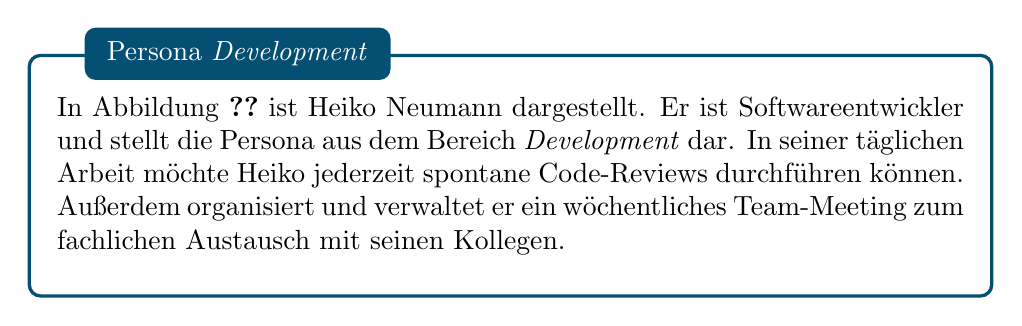
\begin{tikzpicture}
\node [mybox] (box){%
    \begin{minipage}{0.95\textwidth}
        In Abbildung \ref{fig:persona-development} ist Heiko Neumann dargestellt. Er ist Softwareentwickler und stellt die Persona aus dem Bereich \textit{Development} dar. In seiner täglichen Arbeit möchte Heiko jederzeit spontane Code-Reviews durchführen können. Außerdem organisiert und verwaltet er ein wöchentliches Team-Meeting zum fachlichen Austausch mit seinen Kollegen.
    \end{minipage}
};
\node[fancytitle, right=20pt] at (box.north west) { Persona \textit{Development} };
\end{tikzpicture}

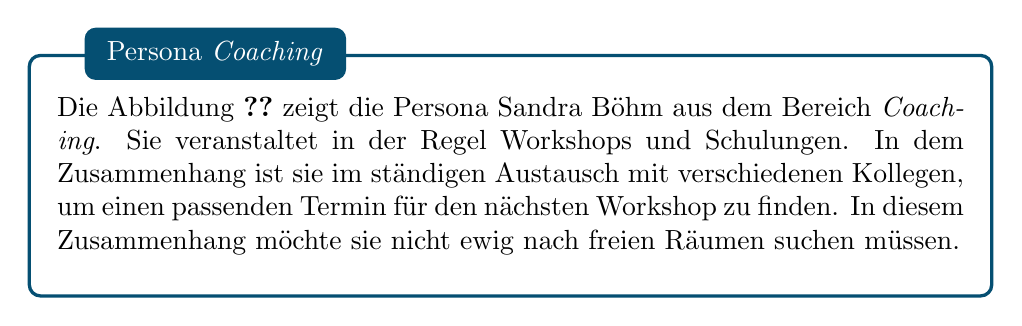
\begin{tikzpicture}
\node [mybox] (box){%
    \begin{minipage}{0.95\textwidth}
        Die Abbildung \ref{fig:persona-coaching} zeigt die Persona Sandra Böhm aus dem Bereich \textit{Coaching}. Sie veranstaltet in der Regel Workshops und Schulungen. In dem Zusammenhang ist sie im ständigen Austausch mit verschiedenen Kollegen, um einen passenden Termin für den nächsten Workshop zu finden. In diesem Zusammenhang möchte sie nicht ewig nach freien Räumen suchen müssen. 
    \end{minipage}
};
\node[fancytitle, right=20pt] at (box.north west) { Persona \textit{Coaching} };
\end{tikzpicture}

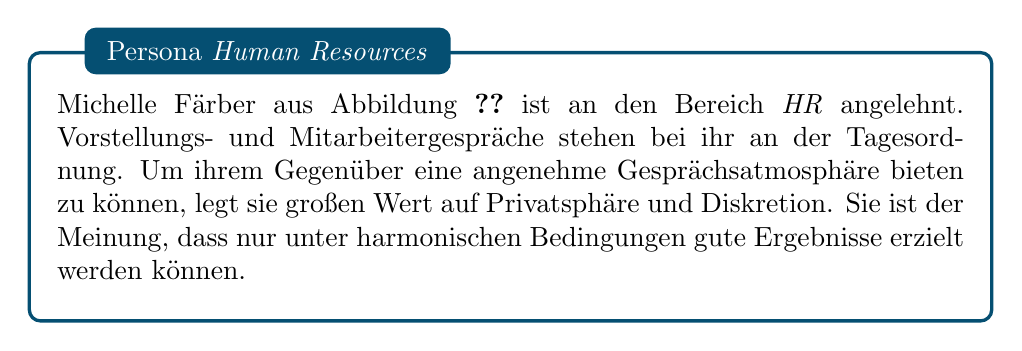
\begin{tikzpicture}
\node [mybox] (box){%
    \begin{minipage}{0.95\textwidth}
        Michelle Färber aus Abbildung \ref{fig:persona-human-resources} ist an den Bereich \textit{\acl{HR}} angelehnt. Vorstellungs- und Mitarbeitergespräche stehen bei ihr an der Tagesordnung. Um ihrem Gegenüber eine angenehme Gesprächsatmosphäre bieten zu können, legt sie großen Wert auf Privatsphäre und Diskretion. Sie ist der Meinung, dass nur unter harmonischen Bedingungen gute Ergebnisse erzielt werden können.
    \end{minipage}
};
\node[fancytitle, right=20pt] at (box.north west) { Persona \textit{Human Resources} };
\end{tikzpicture}

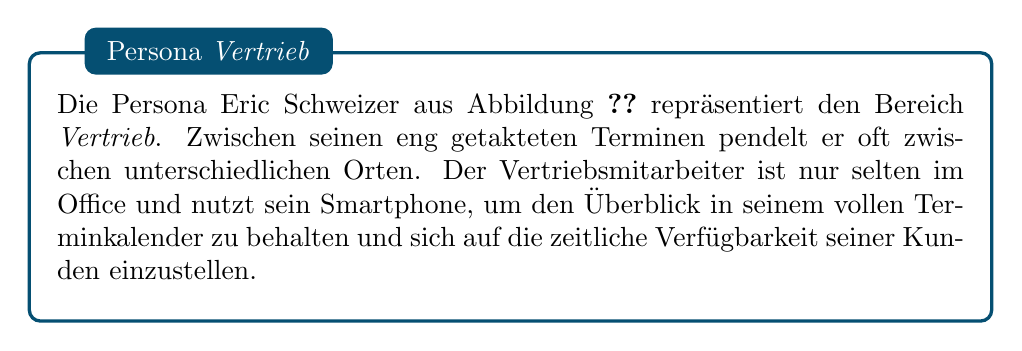
\begin{tikzpicture}
\node [mybox] (box){%
    \begin{minipage}{0.95\textwidth}
        Die Persona Eric Schweizer aus Abbildung \ref{fig:persona-vertrieb} repräsentiert den Bereich \textit{Vertrieb}. Zwischen seinen eng getakteten Terminen pendelt er oft zwischen unterschiedlichen Orten. Der Vertriebsmitarbeiter ist nur selten im Office und nutzt sein Smartphone, um den Überblick in seinem vollen Terminkalender zu behalten und sich auf die zeitliche Verfügbarkeit seiner Kunden einzustellen.
    \end{minipage}
};
\node[fancytitle, right=20pt] at (box.north west) { Persona \textit{Vertrieb} };
\end{tikzpicture}

Durch das Modellieren der Personae auf Grundlage des Fragebogens und der Interviews können wichtige Erkenntnisse gewonnen werden. Die Personae liefern dabei wertvolle Informationen im Zusammenhang mit dem Nutzungskontext und die damit verbundenen Anforderungen an das System. Abschließend konnte hierbei ein guter Eindruck über die Ziele und Wünsche der Nutzer aus den verschiedenen Tätigkeitsfeldern vermittelt werden.

\clearpage
\section{Prototyping}
\label{sec:prototyping}

Prototyping ist eine Methode, bei der so früh wie möglich eine erste, vereinfachte Version (Prototyp) der angestrebten Lösung realisiert wird \cite[S. 25]{fuchs_requirements-engineering_2002}. Diese wird genutzt, um das System zu evaluieren und zu verbessern, noch bevor ein lauffähiges System vorhanden ist. Abhängig vom verfolgten Ziel ist der Prototyp in seinen Eigenschaften mehr oder weniger stark ausgeprägt. Ein Prototyp lässt sich dabei durch die Betrachtung der folgenden Dimensionen charakterisieren. \cite[S. 72-73]{richter_usability_2016}

\begin{itemize}
  \item Der \textit{Funktionsumfang} beschreibt, welche und wie viele Funktionen, bezogen auf den gesamten Umfang, im Prototyp gezeigt werden sollen
  
  \item Als \textit{Funktionstiefe} wird bezeichnet, wie detailliert die einzelnen Funktionen wiedergegeben werden sollen
  
  \item Die \textit{Darstellungstreue} gibt an, wie ähnlich der Prototyp dem Endprodukt in Bezug auf Aussehen und Benutzeroberfläche sein soll
  
  \item Mit der \textit{Interaktivität} wird beschrieben, wie interaktiv der Prototyp sein soll
  
  \item Mit \textit{Datengehalt} ist gemeint, ob reale Daten, Beispiele oder nur Platzhalter für Bezeichnungen zum Einsatz kommen
  
  \item Die \textit{technische Reife} beschreibt, wie viel der endgültigen Technologie im Prototyp verwendet wird
\end{itemize}

In diesem Zusammenhang wird auch oft von \textit{low-fidelity}, \textit{mid-fidelity} und \textit{high-fidelity} Prototypen gesprochen. Diese Begriffe und deren Unterschiede werden daher im Folgenden kurz erläutert.

\begin{itemize}
  \item \textit{low-fidelity:} Dies ist die am einfachsten gehaltene und kostengünstigste Ausprägung eines Prototyps. In den ersten Schritten werden oft einfache Sketches mittels Stift und Papier entworfen. Die Ideen der Entwickler können dabei schnell in eine begreifbare Form gebracht werden. Durch die Visualisierung und Kommunikation ergibt sich ein besseres Verständnis des Produkts.
  
  \item \textit{mid-fidelity:} Oft wird nur zwischen low-fidelity und high-fidelity gesprochen. Ein mid-fidelity Prototyp ist eine Art Zwischenschritt und entspricht einem erweiterten low-fidelity Prototyp. Seine Darstellung ist dabei weiterhin zurückhaltend und größtenteils in schwarz-weiß gehalten. Der Vorteil ist, dass hierbei bereits digitale und interaktive Benutzeroberflächen zum Einsatz kommen. Benötigte Daten oder komplexe Funktionen werden dabei meist vereinfacht oder nur vorgetäuscht.
  
  \item \textit{high-fidelity:} Dieser Prototyp bildet ein interaktives System so ab, wie es tatsächlich sein soll. Das Design ist dabei meist größtenteils ausformuliert, Funktionsumfang oder -tiefe können dagegen noch eingeschränkt sein. Diese Art ist dabei sehr zeit- und ressourcenintensiv, weshalb dabei oft Technologien zum Einsatz kommen, die später auch im Produkt genutzt werden können.
\end{itemize}

Der Prototyp im Rahmen der Konzeption dieser Arbeit wird dabei zwischen low- und mid-fidelity umgesetzt. Der Funktionsumfang soll dabei relativ hoch sein und möglichst viele Szenarien des endgültigen Produkts anbieten. Die Funktionstiefe beschränkt sich dabei eher auf die visuelle Darstellung ohne Anbindung an ein Backend oder ähnliches. Die Darstellung soll bereits in vielen Teilen in die Richtung des Produkts gehen, dabei aber trotzdem dezent wirken. Zudem soll der Prototyp sehr interaktiv sein, um auch tatsächlich den realen Kommunikationsfluss bei der Interaktion zu simulieren. Als Datenmodell werden dabei statische, fiktive Werte zum Einsatz kommen. Technisch gesehen lässt sich für das Endprodukt dabei wenig bis gar nichts nutzen, da der Prototyp in einer komplett anderen Entwicklungsumgebung und Zielplattform entwickelt wird. 

\subsection{Anforderungen}
\label{subsec:anforderungen-prototyp}

Beim prototypischen Aufbau des Chatbots geht es darum zu erkennen, ob eine gewisse Konversationsstruktur oder \ac{UI}-Erweiterung für die User funktioniert und verständlich ist oder nicht. Der Prototyp soll daher die Möglichkeit bieten, Ideen relativ schnell und unkompliziert umsetzen und evaluieren zu können. Ist diese Möglichkeit gegeben, können die erarbeiteten Konzepte sehr früh getestet werden (\textit{test early - fail early}). Der Vorteil ist dabei, dass Probleme frühzeitig erkannt und beseitigt werden können. Kommen diese Fehler erst im späteren Verlauf zum Vorschein, verursachen sie deutlich mehr Aufwand. In Bezug auf einen komplexen Chatbot, der in der Realität von Trainingsdaten und Machine Learning profitiert, muss eine vereinfachte Testumgebung verwendet werden. 

Eine erste Möglichkeit ist dabei das \textit{Paper Prototyping}. Bei dieser low-fidelity Methode wird mit Hilfe von gezeichneten oder gedruckten Komponenten das Verhalten eines zu entwickelnden Systems simuliert. Dabei können vor allem erste, prinzipielle Ideen wie der Aufbau eines User Interfaces und die Anordnung von Labels oder Buttons evaluiert werden. In Bezug auf die Entwicklung eines Chatbots müssen dafür vorgefertigte Textpassagen oder \ac{UI}-Elemente erstellt werden, die dann bei Bedarf genutzt werden können. Ein Vorteil dieser Methode ist sicherlich, dass Skizzen sehr schnell erstellt und angepasst werden können. Außerdem können alle Personen intuitiv damit umgehen. Diese Vorgehensweise erweckt beim Probanden allerdings nicht den Eindruck, dass er ein interaktives oder gar intelligentes System bedient. Daher soll zunächst ein anderer Ansatz verfolgt werden. 

Nachdem als Prototyp kein komplett funktionales System aufgesetzt wird, soll dies mit Hilfe der \textit{\ac{WOz}} Methode umgesetzt werden. Mit \ac{WOz}-Prototypen werden meist komplexe Systemreaktionen durch  einen menschlichen Assistenten simuliert \cite[S. 342]{weber_kompendium_2008}. So können komplexe Dialoge evaluiert werden, bevor überhaupt ein spracherkennendes System implementiert wird. Der menschliche Agent (\acl{WOz}) steuert die Reaktionen des Prototyps auf Basis von Texteingaben des Users. Es muss dazu also keine aufwendige \ac{NLP}-Plattform verwendet oder gar implementiert werden. Dabei geht der \ac{WOz} nach konkreten Regeln vor, die zuvor für das System festgelegt wurden. Ein \ac{WOz}-Test kann gemäß Abbildung \ref{fig:wizard-of-oz-v1} aufgebaut werden.
\newline

\begin{figure}[htb]
    \centering
    \includegraphics[width=0.75\textwidth]{bilder/WizardOfOz_v1.png}
    \caption{Einfaches Prototyping mit der \acl{WOz} Methode}
    \label{fig:wizard-of-oz-v1}
\end{figure}

Dabei sitzt der \acl{WOz} auf der einen, der Test-User und Test-Operator auf der anderen Seite eines Tisches. Der Operator moderiert das Szenario und führt die Testperson durch die Aufgaben. Der User bearbeitet die Aufgaben und sendet seine Anfragen an den \ac{WOz}, der diese nach einem zuvor definierten Ablaufszenario beantwortet. Der Operator kann währenddessen Notizen über die Testdurchführung machen.

Der große Nachteil bei einer Durchführung an diesem Aufbau ist, dass sich alle Beteiligten gegenseitig sehen und hören können. Der \acl{WOz} bekommt also sowohl die Kommunikation zwischen Test-User und Test-Operator, als auch deren Gestiken und Mimiken mit. Er könnte das System durch diese weiteren Informationskanäle daher anders bedienen, als er es bei einer reinen Textanfrage tun würde. Dieses Problem gilt gleichermaßen auch umgekehrt. Wenn die Testperson den \ac{WOz} sieht und realisiert, dass die Antworten von ihm kommen ist die Illusion von der Interaktion mit einem intelligenten System zerstört. \cite{bluemm_designing_2017} 

Diese Probleme lassen sich beheben, wenn der \acl{WOz} in einen Raum, Test-User und Test-Operator in einen anderen Raum platziert werden (siehe Abbildung \ref{fig:wizard-of-oz-v2}).
\newline

\begin{figure}[htb]
    \centering
    \includegraphics[width=0.75\textwidth]{bilder/WizardOfOz_v2.png}
    \caption{Erweitertes Prototyping mit der \acl{WOz} Methode}
    \label{fig:wizard-of-oz-v2}
\end{figure}

Im einfachsten Fall könnte dies mit Hilfe eines \textit{Chat Messengers}, wie z.B. Slack umgesetzt werden. User und Operator sitzen dazu in einem Raum, der \ac{WOz} in einem anderen. Beide haben jeweils ein Fenster des Chat Messengers geöffnet, wodurch sie ihre Nachrichten austauschen können. Die prinzipiellen Anforderungen an getrennte Räume und der Möglichkeit zum Textnachrichten-Austausch sind damit gegeben. Problematisch wird in diesem Zusammenhang aber die Chat-Umgebung an sich. Zunächst könnte der User erkennen, dass es sich um eine standardmäßige Messaging Platform handelt und die Illusion vom intelligenten Chatbot zerstören. Weiterhin sind die Möglichkeiten zur \ac{UI}-Erweiterung begrenzt, wodurch nur ein Bruchteil des Funktionsumfangs getestet werden könnte. Diese Nachteile sollen im nächsten Schritt egalisiert werden.  

Der Test-User soll nun eine prototypische Benutzeroberfläche an einem Rechner bedienen. Seine Eingaben sendet er dabei über eine Netzwerkverbindung direkt an den \ac{WOz}. Nachdem dieser ein Mensch ist, versteht er alle Intentionen des Nutzers und kann diese entsprechend zuordnen. Dabei geht er nach festgelegten Regeln vor und sendet die Antworten zurück an den User. Diese Antworten tippt er nicht selbst, sondern bedient sich dabei an vorgefertigten Phrasen, Textpassagen oder \ac{UI}-Elementen. Diese unterscheiden sich dabei je nach Szenario oder Intention des Nutzers. Bei einer übersichtlichen Gestaltung der Benutzeroberfläche findet sich der \acl{WOz} auch bei komplexen Tests zurecht. 

\subsection{Prototyping Tool}
\label{subsec:prototyping-tool}

Um all diese Anforderungen umsetzen zu können, wird ein \textit{\ac{cpt}} verwendet\footnote{Die Arbeit im Prototyping Tool stammt vom \ac{CUI}-Team der \adorsys\ unter der Leitung von Steffen Blümm}. Umgesetzt wird dies mit \textit{Max} von \textit{Cycling74}. Max ist eine grafische Entwicklungsumgebung, in der Module in einer Art \textit{Baukastensystem} verbunden werden. Die Entwicklung und Implementierung in diesem Zusammenhang ist nicht Bestandteil dieser Arbeit und soll daher nicht weiter beschrieben werden. Das Prototyping-System wird im Rahmen der Arbeit zur konzeptionellen Überprüfung der Konversationsstruktur und der \ac{UI}-Elemente genutzt. Wichtig zu erwähnen ist in diesem Zusammenhang, dass es gemäß der vorherigen Überlegungen zwei Benutzeroberflächen (Panels) gibt. Eine der Benutzeroberflächen bedient der \acl{WOz}, die andere der Test-User. Wie bereits zuvor festgelegt, befinden sich die jeweiligen Rechner in verschiedenen Räumen und tauschen ihre Daten über eine Netzwerkverbindung aus. 
\newline

\begin{figure}[H]
    \centering
    \includegraphics[width=0.75\textwidth]{bilder/WizardOfOz_v3.png}
    \caption{Komplettaufbau des Prototypings mit der Wizard of Oz Methode}
    \label{fig:wizard-of-oz-v3}
\end{figure}

Mit dem \textit{Tester-Panel} interagiert in der Regel nur der Test-User. Es ist dafür zuständig, dass die vom Nutzer eingegebenen Textanfragen übertragen werden. Seine Textnachrichten kann der User über die dunkelgraue Leiste am unteren Rand eingeben und abschicken. Außerdem gibt dieses Panel die vom \acl{WOz} generierten Antworten aus. Diese können, wie schon im vorherigen Teil der Arbeit beschrieben, sowohl Textnachrichten als auch erweiterte \ac{UI}-Elemente sein. Ziel dieser prototypischen User-Tests ist herauszufinden, welche erweiterten \aclp{UI} für den Nutzer verständlich sind und ihn bei der Raumbuchung unterstützen. Die entsprechenden \ac{UI}-Elemente können dann interaktiv bedient werden. Ein beispielhafter Ausschnitt des Tester-Panels ist in Abbildung \ref{fig:tester-panel} dargestellt. Eine ausführliche Darstellung aller \ac{UI}-Elemente befindet sich aus Gründen der besseren Lesbarkeit im Anhang \ref{sec:anhang-ui-elemente-prototyping}.
\newline

\begin{figure}[H]
    \centering
    \includegraphics[width=0.8\textwidth]{bilder/TesterPanel.png}
    \caption{Grafische Benutzeroberfläche des Tester-Panels}
    \label{fig:tester-panel}
\end{figure}

Der \ac{WOz} sitzt während der Durchführung vor dem \textit{Simulator-Panel}. Diese Benutzeroberfläche kann gemäß eines vorher definierten Szenarios dynamisch aufgebaut werden. Dabei kann auf vordefinierte Phrasen oder \ac{UI}-Elemente zurückgegriffen werden. Zudem blinkt ein kleiner Kreis oben links, sobald der User auf der Tastatur tippt. Sendet er eine Nachricht ab, erscheint diese ebenfalls in der oberen linken Ecke. Durch das Triggern der Nachrichten wird Zeit gespart, da der \ac{WOz} nicht jede Antwort selbst generieren und formulieren muss. Außerdem ist so die Möglichkeit gegeben, dass jeder User innerhalb eines bestimmten Szenarios die gleichen Antworten und Formulierungen erhält, wodurch eine Verfälschung der Testergebnisse verhindert wird. Die Benutzeroberfläche des Simulator-Panels ist in Abbildung \ref{fig:simulator-panel} dargestellt.
\newline

\begin{figure}[H]
    \centering
    \includegraphics[width=1.0\textwidth]{bilder/simulator-panel.png}
    \caption{Grafische Benutzeroberfläche des Simulator-Panels}
    \label{fig:simulator-panel}
\end{figure}

Um ein \textit{Szenario} mit den verschiedenen Intents und Responses zu erstellen, wird eine Art \textit{Skript} verwendet. Dieses Skript wird im Format \textit{\ac{JSON}} geschrieben und enthält die entsprechenden Elemente in strukturierter Form. Für jedes Szenario gibt es dabei einen eigenen Tab (Tabs sind nicht in der Abbildung \ref{fig:simulator-panel} ersichtlich). 

Innerhalb jedes Szenarios können dann \textit{Intents} (blaue Rahmen) angelegt werden. Die ersten beiden Intents jedes Szenarios heißen \textit{helpIntent} und \textit{errorIntent}. Diese sind zum Schnellzugriff in der oberen Leiste (gelbes und oranges Feld) und triggern einfache Textnachrichten. Jeder Intent ist gleichermaßen aufgebaut und enthält die Parameter \textit{name}, \textit{utterances} und \textit{responses} (siehe Abbildung \ref{fig:json-structure}). 

Mit dem Parameter \textit{name} kann dem Intent ein Überbegriff zugeordnet werden. Unter \textit{utterances} können einige Beispielsätze des Users aufgezählt werden, die dem Operator das Bedienen erleichtern. Der letzte Parameter \textit{responses} kann je nach Art der Nachricht sehr umfangreich werden. 

Jede Response hat einen Parameter \textit{subject}, mit dem ihr ein Name zugeordnet werden kann. Mit Hilfe einer \textit{phrase} wird angegeben, welche Textnachricht an den User gesendet wird. Mit einem \textit{hint} kann dieser Text darunter zusätzlich in kleinerer Schrift ergänzt werden. Die Werte für \textit{type} und \textit{tags} ordnen der Response ein entsprechendes \ac{UI}-Element zu. Dabei gibt es verschiedene Elemente, wie z.B. eine \textit{CalendarView}, eine \textit{CollectionView} oder unterschiedliche \textit{Slidebars}. Mit Hilfe des Parameters \textit{payload} können dann zusätzliche Informationen über Startzeit, Dauer, Datum oder Raumname mitgegeben werden. An dieser Stelle soll aus Gründen der Übersichtlichkeit auf eine umfangreiche Darstellung verzichtet werden. Stattdessen ist nachfolgend zur beispielhaften Darstellung der Struktur einer Response die Implementierung einer kurzen \textit{Textmessage} in Listing \ref{lst:szenario-json} dargestellt. 
\newline

\begin{figure}[H]
    \centering
    \includegraphics[width=1\textwidth]{bilder/json-structure-v2.PNG}
    \caption{Struktur eines Szenarios im \acs{JSON}-Format}
    \label{fig:json-structure}
\end{figure}
\clearpage
\begin{lstlisting}[caption={Beispielhafte Response im \acs{JSON}-Format}, captionpos=b, label={lst:szenario-json}, language=myjson]
{
    "responses": [
    {
        "subject": "Help",
        "phrase": "Ich bin dein persoenlicher Raumbuchungs Assistent. Ich helfe dir gerne dabei, einen Besprechungsraum fuer deine Termine zu finden und zu buchen.",
        "type": "textmessage"
    }]
}

\end{lstlisting}

\subsection{Usability Testessen}
\label{subsec:usability-testessen}

Erste User Tests mit dem \textit{Prototyping Tool} konnten mit externen Nutzern im Rahmen eines so genannten \textit{Usability Testessens}\footnote{www.usability-testessen.org} durchgeführt werden. Bei dieser Veranstaltung bringen Entwickler ihre Prototypen, Websites oder Apps mit. Freiwillige, vom Produkt unabhängige Nutzer testen diese dann auf ihre Gebrauchstauglichkeit. Dies hat den Vorteil, dass die Nutzer in der Regel keinen Bezug zum Produkt haben und somit ein unvoreingenommenes und ehrliches Feedback abgeben. 

Die Veranstalter selbst bezeichnen das als \textit{Speedtesting}. Die Probanden testen die verschiedenen Produkte in sechs Runden à zwölf Minuten. Nach Ablauf einer Runde wandern die Tester zum nächsten Stand. Getestet wird dabei mit Hilfe der \textit{Thinking-Aloud-Methode}. Dabei wird der Teilnehmer während der Testsitzung angehalten zu äußern, was er gerade denkt oder fühlt. Die Methode liefert somit ein schnelles Feedback und hilft, Usability-Probleme zu identifizieren. Um sicherzustellen, dass keine Informationen verloren gehen, wird der User Test mit einem Aufnahmegerät aufgezeichnet. Eine entsprechende Einverständniserklärung wird jedem Teilnehmer vor Beginn des Tests zur Unterschrift vorgelegt. Diese ist im Anhang \ref{sec:anhang-einverstaendniserklaerung-feedback-ext} zu finden. 

Der Testdurchlauf besteht im Wesentlichen aus zwei Teilen. Zunächst wird der Proband gebeten, ein bestimmtes Szenario mit Hilfe des Protoyping Tools abzuarbeiten. Als Benutzeroberfläche steht ihm dabei das Tester-Panel (vgl. Abbildung \ref{fig:tester-panel}) zur Verfügung. Alle seine Anfragen werden über eine Netzwerkverbindung an den \acl{WOz} gesendet, der vordefinierte Antworten über das Simulator-Panel (vgl. Abbildung \ref{fig:simulator-panel}) auswählen kann. Dem Proband wird somit der Eindruck einer Interaktion mit einem intelligenten Chatbot vorgetäuscht, hinter dem in Wirklichkeit ein Mensch steckt. Während der Nutzer das Szenario bearbeitet, können dank der Thinking-Aloud-Methode wertvolle Notizen zu Wahrnehmung und Verhalten des Nutzers gemacht \mbox{werden}. 

\begin{tikzpicture}
\node [mybox] (box){%
    \begin{minipage}{0.95\textwidth}
        Beschreibung:\\
        \textit{„Du willst morgen Vormittag um 10 Uhr an einem Meeting (Skype) teilnehmen, das bis zu 2 Stunden dauern kann. Die Videokonferenz findet an deinem eigenen Rechner statt. Um deine Kollegen nicht zu stören, willst du nicht vom Arbeitsplatz, sondern von einem Besprechungsraum aus teilnehmen. }\\
        Aufgabe:\\
        \textit{Lasse dir die verfügbaren Räume anzeigen und reserviere anschließend den Raum R2 von 10 bis 12 Uhr.“}
    \end{minipage}
};
\node[fancytitle, right=20pt] at (box.north west) { Szenario \textit{Usability Testessen} };
\end{tikzpicture}

Ist das Szenario erfolgreich abgeschlossen, wird der User noch gebeten, einen \textit{Feedback-Fragebogen} auszufüllen. Dieser besteht aus elf Gegensatzpaaren hinsichtlich der Wahrnehmung und Einstellung des Nutzers zum Produkt. Die Fragen sind dabei durch eine Skala mit fünf Auswahlmöglichkeiten zu beantworten. Eine Übersicht der Kriterien des Feedback-Fragebogens ist in der nachfolgenden Liste dargestellt.

\begin{itemize}
    \setlength{\itemindent}{0.5cm}
    \item verständlich $\longleftrightarrow$ unverständlich
    \item leicht zu erlernen $\longleftrightarrow$ schwer zu erlernen
    \item schnell $\longleftrightarrow$ langsam
    \item aufgeräumt $\longleftrightarrow$ überladen
    \item unterstützend $\longleftrightarrow$ behindernd
    \item angenehm $\longleftrightarrow$ unangenehm
    \item einfach $\longleftrightarrow$ kompliziert
    \item sympathisch $\longleftrightarrow$ unsympathisch
    \item erwartungskonform $\longleftrightarrow$ nicht erwartungskonform 
    \item effizient $\longleftrightarrow$ ineffizient 
    \item übersichtlich $\longleftrightarrow$ verwirrend 
\end{itemize}

Eine ausführliche Auflistung der Fragebögen mit Notizen zu den jeweiligen Teilnehmern befindet sich im Anhang \ref{sec:anhang-feedback-ext}. Die Inhalte und deren durchschnittliche Bewertung sind in Abbildung \ref{fig:diagram-auswertung-usability-testessen} anhand eines Diagramms dargestellt. Die gelbe Referenzlinie zeigt die durchschnittliche Bewertung des Systems durch alle Probanden. 
\newline

\begin{figure}[H]
    
  \begin{tikzpicture}

      \definecolor{myblue}{HTML}{0984bf} % Sekundäres adorsys blau
      \definecolor{myyellow}{HTML}{eed525} % adorsys gelb
      
      \draw (0cm,0cm) -- (13.2cm,0cm);  % Achse horizontal (Abzisse)
      \draw (0cm,0cm) -- (0cm,-0.1cm);  % linkes Ende der Abzisse
      \draw (13.2cm,0cm) -- (13.2cm,-0.1cm);  % rechtes Ende der Abzisse
      
      \draw (-0.1cm,0cm) -- (-0.1cm,10.5cm);  %Achse vertikal (Ordinate)
      \draw (-0.1cm,0cm) -- (-0.2cm,0cm);  % unteres Ende der Ordinate
      \draw (-0.1cm,10.5cm) -- (-0.2cm,10.5cm) node [left] {\%};  % oberes Ende der Ordinate
    
      % Hilfslinien bei 10, 20, ..., 90, 100 mit Beschriftung
      \foreach \x in {10,20,30,40,50,60,70,80,90,100}
        \draw[gray!50, text=black] (-0.2 cm,\x mm) -- (13.2 cm,\x mm) % Zeichnen der Hilfslinien
            node at (-0.5 cm,\x mm) {\x}; % Beschriftung der Hilfslinien
    
      % Gelber Strich, Avergave
      \draw[line width=0.5mm, myyellow] (-0.1 cm,80 mm) -- (13.1 cm,80 mm); % Zeichnen der Hilfslinien
      
      %\node at (6.7cm,11cm) {Zustimmung in Prozent};  %Überschrift
    
      \foreach \pos/\index in     {0.3/1,  % \pos ist Position der Säulen
                                  1.5/2,  % \index zählt bis 11 hoch
                                  2.7/3,
                                  3.9/4,
                                  5.1/5,
                                  6.3/6,
                                  7.5/7,
                                  8.7/8,
                                  9.9/9,
                                  11.1/10,
                                  12.3/11}
        {
        
        % Datensatz 'values' lesen -> Aus Index das jeweilige Kriterium und den Wert lesen
        \DTLassign{valuesTestEssen}{\index}{\kriterium=kriterium,\wert=wert}
        
         \draw[fill=myblue] (\pos cm,0cm) rectangle (0.6cm+\pos cm,\wert mm) % die Säulen
           node at (0.3cm + \pos cm,\wert mm + 0.3cm) {\wert}; %die Prozente über den Säulen
         \node[text=white, rotate=90, right] at (0.3 cm +\pos cm,0.5cm) {\textbf{\kriterium}}; %Säulenbeschriftung
        };
        
    \end{tikzpicture}
    \caption{Ergebnisse des Usability Testessens}
    \label{fig:diagram-auswertung-usability-testessen}
\end{figure}

Im Großen und Ganzen gaben die Probanden positives Feedback. Im Durchschnitt ergibt sich eine Zustimmung zum System von ca. 80\,\%. Insgesamt gibt es dabei keine allzu großen Diskrepanzen. Anzumerken ist, dass ein Großteil der Nutzer den Prototyp als \textit{angenehm} (88\,\%), \textit{verständlich} und \textit{schnell} (je 83\,\%) empfand. Etwas weniger, aber dennoch 75\,\% Zustimmung bekamen Kriterien wie \textit{aufgeräumt} oder \textit{übersichtlich}, was jedoch auch auf die prototypische Umgebung zurückzuführen sein kann. Anzumerken ist hierbei, dass aufgrund von begrenzter Zeit und Umfang dieser Testveranstaltung keine fundierte Aussage über qualitative oder funktionale Eigenschaften des Systems getroffen werden kann. Die Bewertung ist jedoch äußerst hilfreich, um ein erstes, schnelles Feedback der geplanten Applikation zu erhalten und hilft damit bei der weiteren Konzeption des Systems.

Die ersten Ergebnisse spiegeln sich auch mit einigen Zitaten der Probanden wider. \textit{„Wenn das bei uns so einfach funktionieren würde, wäre das schon toll.“} oder \textit{„Das hätte ich auch gerne, ich kenne das komplizerter.“} sind nur einige Zitate in diesem Zusammenhang. Daraus lässt sich ableiten, dass die Nutzer dem System grundsätzlich positiv gegenüberstehen und sowohl die Raumbuchung via Chatbot als auch die \ac{UI}-Erweiterungen verständlich sind. 

Von beinahe allen Probanden wurde außerdem erwähnt, dass das Feature \textit{Chatbot is thinking} hilfreich ist und den Chatbot obendrein sympathisch macht. Mit dieser Funktion wird die Zeit überbrückt, die der Chatbot für die Verarbeitung einer Nutzereingabe benötigt. Als negatives Feedback erwähnten einige User die farblichen Markierungen im Lageplan. Hier geht die farbliche Markierung des gebuchten Raumes gegenüber den anderen Symbolen unter. Abgesehen davon war der Lageplan jedoch hilfreich. Als Anmerkung nannten die Nutzer immer wieder die Frage nach der Ausstattung der Räume. Hier spielten vor allem die Fragen nach WLAN, Anzahl der Plätze, Whiteboard, Flipchart, Beamer, Getränke oder Catering eine Rolle. Zudem äußerten einige User den Wunsch, dass der gebuchte Termin anschließend automatisch in ihren elektronischen Kalender eingetragen werden soll.    

\subsection{Szenarien}
\label{subsec:szenarien}

Im Rahmen von ausführlichen User Tests werden verschiedene Szenarien, basierend auf die erdachten Personae aus \ref{subsec:personae}, entwickelt. Entsprechend den jeweiligen Bereichen Development, Coaching, Human Resources und Vertrieb wird jeweils ein spezifisches Szenario erstellt. Die Szenarien werden im Folgenden kurz vorgestellt und deren Hintergedanken beschrieben.

Das Szenario aus dem Bereich \textit{Development} ist an die Persona Heiko Neumann angelehnt. Heiko ist Softwareentwickler und möchte zusammen mit einem Kollegen ein spontanes Code-Review durchführen. Er hat dabei keine besonderen Ansprüche an einen Raum. Für seine Buchung wird die entsprechende Raumhierarchie aus \ref{tab:raum-priorisierung} \mbox{angewendet}. 

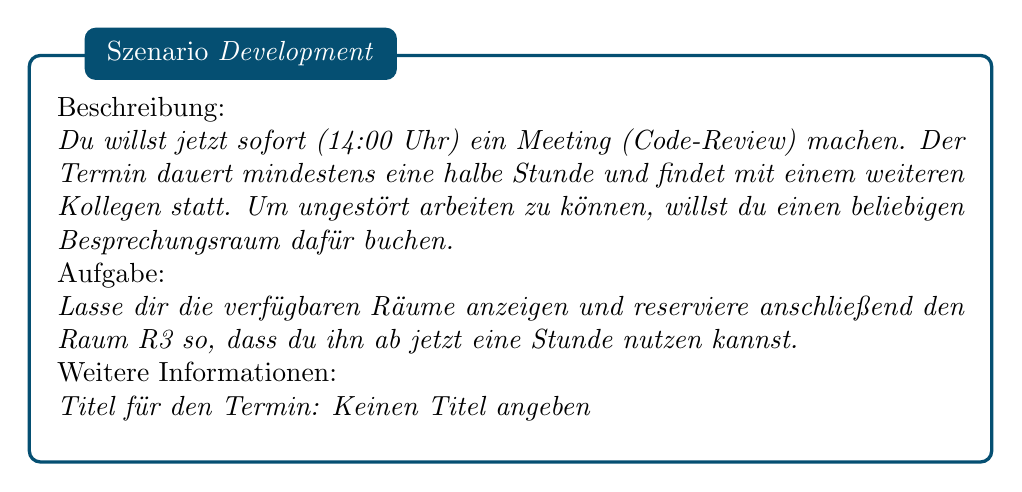
\begin{tikzpicture}
\node [mybox] (box){%
    \begin{minipage}{0.95\textwidth}
        Beschreibung: \\
        \textit{Du willst jetzt sofort (14:00 Uhr) ein Meeting (Code-Review) machen. Der Termin dauert mindestens eine halbe Stunde und findet mit einem weiteren Kollegen statt. Um ungestört arbeiten zu können, willst du einen beliebigen Besprechungsraum dafür buchen.} \\
        Aufgabe: \\
        \textit{Lasse dir die verfügbaren Räume anzeigen und reserviere anschließend den Raum R3 so, dass du ihn ab jetzt eine Stunde nutzen kannst.} \\
        Weitere Informationen: \\
        \textit{Titel für den Termin: Keinen Titel angeben}
    \end{minipage}
};
\node[fancytitle, right=20pt] at (box.north west) { Szenario \textit{Development} };
\end{tikzpicture}

Sandra Böhm ist die Persona aus dem Bereich \textit{Coaching}. Sie möchte einen interaktiven Scrum Workshop veranstalten. Aufgrund der Teilnehmerzahl von zwölf Personen benötigt sie dazu den Raum R6. Das System soll dabei erkennnen, dass es sich um einen ganztägigen Termin handelt und bei der Buchung, entsprechend der Idee aus \ref{subsec:interviews}, nach Vor- und Nachbereitungszeit für den Termin fragen. Wählt der User eine entsprechende Vor- und Nachbereitungszeit aus, nimmt das System direkt alle drei Buchungen vor und erleichtert dem Nutzer somit die Buchung von drei einzelnen Terminen. 

\begin{tikzpicture}
\node [mybox] (box){%
    \begin{minipage}{0.95\textwidth}
        Beschreibung: \\
        \textit{Du willst einen interaktiven Scrum Workshop halten. Daran werden etwa zwölf Leute teilnehmen, weshalb du den Raum R6 benötigst. Der Termin soll als ganztägiges Ereignis stattfinden. Die Kernzeit für alle Teilnehmer ist dabei von 9:00 Uhr bis 17:00 Uhr. Für dich selbst möchtest du jedoch zusätzlich je eine Stunde zur Vor- und Nachbereitung des Workshops buchen.} \\
        Aufgabe: \\
        \textit{Lasse dir die nächsten Termine anzeigen, an denen der Raum R6 ganztägig frei ist und reserviere ihn anschließend für den nächstmöglichen Zeitpunkt zu den oben stehenden Bedingungen.} \\
        Weitere Informationen: \\
        \textit{Titel für den Termin: „Scrum Workshop“}
    \end{minipage}
};
\node[fancytitle, right=20pt] at (box.north west) { Szenario \textit{Coaching} };
\end{tikzpicture}

Die Persona Michelle Färber repräsentiert den Bereich \textit{Human Resources}. In dem spezifischen Szenario möchte sie einen Raum für ein Vorstellungsgespräch buchen. Wird dem System entsprechend mitgeteilt, dass es sich um ein Vorstellungsgespräch handelt, ändert sich die Priorisierung der Räume. Räume, die Diskretion bieten, werden in diesem Fall höher priorisiert und zuerst vorgeschlagen. 

\begin{tikzpicture}
\node [mybox] (box){%
    \begin{minipage}{0.95\textwidth}
        Beschreibung: \\
        \textit{Du arbeitest im Bereich HR und möchtest einen Raum für ein Vorstellungsgespräch buchen. Du hast mit dem Bewerber einen Termin am nächsten Montag von 10:00 Uhr bis 11:30 Uhr vereinbart. Da du als HR-Mitarbeiter möchtest, dass der Bewerber sich wohlfühlt und möglichst ein gewisses Maß an Diskretion gegeben ist, ergibt sich für dich folgende Priorisierung der Räume: R4 (Diskretion, hell), R3 (Diskretion, dunkel), R1 (keine Diskretion, hell), R2 (keine Diskretion, hell). } \\
        Aufgabe: \\
        \textit{Reserviere den bestmöglichen Raum zu den oben genannten Bedingungen.}  \\
        Weitere Informationen: \\
        \textit{Titel für den Termin: „VG Java Entwickler“}
    \end{minipage}
};
\node[fancytitle, right=20pt] at (box.north west) { Szenario \textit{Human Resources} };
\end{tikzpicture}

Eric Schweizer steht für die Persona aus dem \textit{Vertrieb}. Er möchte für die kommende Woche ein Projektanbahnungsgespräch organisieren. Die Uhrzeit ist durch den Kunden fest vorgegeben. Er benötigt dazu keinen besonderen Raum. Für seine Buchung wird die entsprechende Raumhierarchie aus Tabelle \ref{tab:raum-priorisierung} angewendet. 

\begin{tikzpicture}
\node [mybox] (box){%
    \begin{minipage}{0.95\textwidth}
        Beschreibung: \\
        \textit{Du willst nächste Woche am Dienstag ein Projektanbahnungsgespräch organisieren. Zu dem Termin kommen neben dir noch ein Designer, der vorgesehene Projektmanager sowie drei Mitarbeiter des Kunden. Das Meeting soll um 9:30 Uhr beginnen und etwa 2-3 Stunden dauern.} \\
        Aufgabe: \\
        \textit{Lasse dir die verfügbaren Räume anzeigen und reserviere anschließend den Raum R1 von 9:30 Uhr bis 13:00 Uhr.} \\
        Weitere Informationen: \\
        \textit{Titel für den Termin: „Projektanbahnung VR Bank“}
    \end{minipage}
};
\node[fancytitle, right=20pt] at (box.north west) { Szenario \textit{Vertrieb} };
\end{tikzpicture}




\subsection{Workflow}
\label{subsec:workflow}

Zu den beschriebenen Szenarien werden User Tests durchgeführt. Der damit verbundene Workflow und die Grundüberlegungen sollen im Folgenden anhand eines spezifischen Szenarios erläutert werden. Für diesen Fall wird das Szenario aus dem Bereich \textit{Vertrieb} betrachtet. 

Um diese Aufgabe zu erledigen und den Raum R1 von 9:30 Uhr bis 13:00 Uhr zu reservieren, hat der Nutzer verschiedene Möglichkeiten. Diese sind in Abbildung \ref{fig:decision-tree-vertrieb} in Form eines Entscheidungsbaums (engl. \textit{decision tree}) dargestellt. Die einzelnen Zweige werden anschließend genauer erläutert.
\newline

\begin{figure}[H]
    \centering
    \includegraphics[width=0.9\textwidth]{bilder/SzenarioVertriebMindMap.png}
    \caption{Entscheidungsbaum zum Szenario \textit{Vertrieb}}
    \label{fig:decision-tree-vertrieb}
\end{figure}

Zunächst kann sich der Nutzer die ab 9:30 Uhr verfügbaren Räume anzeigen lassen (linker Zweig). Eine entsprechende Formulierung könnte so aussehen:

\begin{center}
    \textit{Welche Räume sind am Dienstag ab 9:30 Uhr frei?}
\end{center}

Das System zeigt daraufhin eine \textit{CalendarView} mit den verfügbaren Räumen. Der Nutzer wählt einen für seinen Zeitraum passenden Zeitslot aus und wird anschließend mit Hilfe von zwei \textit{Slidern} nach der Startzeit und Dauer seines Termins gefragt. Danach hat das System alle notwendigen Parameter und kann die Buchung nach Eingabe eines Titels abschließen.

Bei anderer Formulierung der Intention kann das System direkt erkennen, dass der Nutzer einen Raum von 9:30 Uhr bis 13:00 Uhr benötigt (mittlerer Zweig). Diese Formulierung könnte beispielsweise so lauten:

\begin{center}
    \textit{Ich brauche am Dienstag von 9:30 Uhr bis 13:00 Uhr einen Raum.}
\end{center}

Das System erkennt direkt den Start- und Endzeitpunkt des Termins und kann die verfügbaren Räume mit Hilfe einer \textit{CollectionView} anzeigen. Wählt der Nutzer einen Raum aus, hat das System alle notwendigen Parameter und kann mit der Eingabe des Titels fortfahren. 

Ist die Formulierung ähnlich, beinhaltet allerdings nur den Startzeitpunkt von 9:30 Uhr für den Termin, kann mit einem kleinen Umweg genauso vorgegangen werden (rechter Zweig). Eine Möglichkeit der Formulierung wäre:

\begin{center}
    \textit{Ich möchte am Dienstag um 9:30 Uhr einen Raum buchen.}
\end{center}

Das System fragt den Nutzer über einen \textit{Slider} nach der Dauer des Termins. Hat der User diese eingegeben, kann auf gleiche Art und Weise vorgegangen werden. Der Raum wird über eine \textit{CollectionView} ausgewählt und die Buchung anschließend \mbox{abgeschlossen}. 

Der Abschluss einer Buchung trifft sich für alle möglichen Zweige an einem Punkt wieder. In diesem Szenario ist das die Stelle, an der die \textit{Eingabe des Titels} erfolgt. Im Rahmen der Arbeit wird eine Festlegung zur Angabe von Titeln bei Terminen getroffen. Ab einer Dauer des Termins von 1,5 Stunden muss ein Termin einen Titel haben. Dauert der Termin weniger als 1,5 Stunden, kann der Nutzer optional und auf eigenen Wunsch einen Titel hinzufügen. Tut er dies nicht, wird ein automatisch generierter Titel mit dem Namen des Organisators eingetragen. Anschließend wird die Buchung noch über das \ac{UI}-Element \textit{ConfirmBooking} abgeschlossen.
\clearpage
Der \acl{WOz} hat die in \ref{subsec:prototyping-tool} beschriebene Operator-Ansicht. Die Zweige des oben beschriebenen Entscheidungsbaums sind in Abbildung \ref{fig:operator-screen-vertrieb} als blaue Kästen wieder zu finden. 
\newline

\begin{figure}[H]
    \centering
    \includegraphics[width=1.0\textwidth]{bilder/OperatorSzenarioVertrieb.png}
    \caption{Benutzeroberfläche des Operators zum Szenario \textit{Vertrieb}}
    \label{fig:operator-screen-vertrieb}
\end{figure}

Die linken drei Kästen können entsprechend von oben nach unten abgearbeitet werden. Danach befindet sich der Knotenpunkt zur Eingabe des Titels. Ab hier ist der Ablauf für alle Fälle gleich, wonach der rechte blaue Kasten von oben nach unten durchlaufen wird. 

Der Test-User bekommt von all dem nicht viel mit. Er bearbeitet das Szenario und wählt eine für ihn passende Formulierung aus. Über die Benutzeroberfläche des Tester-Panels interagiert er mit dem System und erhält entsprechende Rückmeldungen in Form von Text oder \ac{UI}-Elementen. Ein möglicher Durchlauf aus der Sicht des Probanden ist in Abbildung \ref{fig:test-user-screen-vertrieb} dargestellt.
\newline

\begin{figure}[H]
    \centering
    \includegraphics[width=0.85\textwidth]{bilder/WorkflowTesterPanel.png}
    \caption{Benutzeroberfläche des Probanden zum Szenario \textit{Vertrieb}}
    \label{fig:test-user-screen-vertrieb}
\end{figure}

\subsection{User Tests}
\label{subsec:user-tests}

Zur Evaluierung der konzeptionellen Überlegungen werden abschließend User Tests durchgeführt. Grundsätzlich sollen dabei Parallelen zu den ersten Tests im Rahmen des Usability Testessens (siehe \ref{subsec:usability-testessen}) gezogen werden können. Daher wird der Prototyp auch in diesem Fall von sechs Probanden getestet. Aufgrund der intensiveren Betrachtungen im Kontext des Requirements Engineering in Form von Fragebögen, Interviews oder der Entwicklung von Personae fällt der Test in diesem Fall umfangreicher aus. Die Probanden bearbeiten jedes der in \ref{subsec:szenarien} definierten Szenarien als eigenständige Aufgabe. Auch hier wird wieder die \textit{Thinking-Aloud-Methode} angewendet und der User Test mit einem Aufnahmegerät aufgezeichnet. Dazu wird die entsprechende Einverständniserklärung aus Anhang \ref{sec:anhang-einverstaendnis-user-test} verwendet. 

Nach der Begrüßung und Unterschrift der Einveständniserklärung bearbeitet der Proband die vier Szenarien in einer zuvor festgelegten Reihenfolge. Nachdem die Nutzer bereits nach wenigen Arbeitsschritten die Bedienung des Systems erlernen, werden die Szenarien unterschiedlich angeordnet, um so eine Verfälschung der Ergebnisse auszuschließen. Dazu werden die vier Szenarien für die User mit Hilfe eines Online-Tools randomisiert \cite{jumk.de_generator_2018}. In Tabelle \ref{tab:szenarien-randomisierung} ist die unterschiedliche Reihenfolge der Szenarien und die jeweils dazugehörige, anonymisierte User-\acs{ID} dargestellt.
\newline

\begin{table}[!htb]
\centering
 \begin{tabular}{ | C{3cm} || C{1.5cm} || C{1.5cm} || C{1.5cm} || C{1.5cm} |} 
 \hline
 User-\acs{ID} & 1 & 2 & 3 & 4  \\
 \hhline{=::====}
 \hline user1723 & HR01 & V01 & D01 & C01 \\ 
 \hline user2626 & D01 & V01 & C01 & HR01 \\ 
 \hline user5156 & C01 & V01 & HR01 & D01 \\ 
 \hline user7027 & V01 & C01 & HR01 & D01 \\ 
 \hline user9337 & V01 & D01 & HR01 & C01 \\ 
 \hline user9716 & C01 & D01 & V01 & HR01 \\ 
 \hline
\end{tabular}
\caption{Randomisierung der Szenarien}
\label{tab:szenarien-randomisierung}
\end{table}

Nach erfolgreicher Durchführung aller Szenarien füllt der Proband den bereits in \ref{subsec:usability-testessen} beschriebenen Feedback-Fragebogen aus. Eine ausführliche Auflistung der Fragebögen mit Notizen zu den jeweiligen Teilnehmern befindet sich im Anhang \ref{sec:anhang-feedback-user-tests}. 

Im Folgenden werden die Ergebnisse des Feedback-Fragebogens in Abbildung \ref{fig:diagram-auswertung-user-test} dargestellt und bewertet. Die gelbe Referenzlinie zeigt die durchschnittliche Bewertung des Systems durch alle User. 
\newline

\begin{figure}[htb]
    
  \begin{tikzpicture}

      \definecolor{myblue}{HTML}{0984bf} % Sekundäres adorsys blau
      \definecolor{myyellow}{HTML}{eed525} % adorsys gelb
     
      \draw (0cm,0cm) -- (13.2cm,0cm);  % Achse horizontal (Abzisse)
      \draw (0cm,0cm) -- (0cm,-0.1cm);  % linkes Ende der Abzisse
      \draw (13.2cm,0cm) -- (13.2cm,-0.1cm);  % rechtes Ende der Abzisse
      
      \draw (-0.1cm,0cm) -- (-0.1cm,10.5cm);  %Achse vertikal (Ordinate)
      \draw (-0.1cm,0cm) -- (-0.2cm,0cm);  % unteres Ende der Ordinate
      \draw (-0.1cm,10.5cm) -- (-0.2cm,10.5cm) node [left] {\%};  % oberes Ende der Ordinate
    
      % Hilfslinien bei 10, 20, ..., 90, 100 mit Beschriftung
      \foreach \x in {10,20,30,40,50,60,70,80,90,100}
        \draw[gray!50, text=black] (-0.2 cm,\x mm) -- (13.2 cm,\x mm) % Zeichnen der Hilfslinien
            node at (-0.5 cm,\x mm) {\x}; % Beschriftung der Hilfslinien
    
       % Gelber Strich, Avergave
      \draw[line width=0.5mm, myyellow] (-0.1 cm, 83 mm) -- (13.1 cm, 83 mm); % node [right] {\o} 
    
      %\node at (6.7cm,11cm) {Zustimmung in Prozent};  %Überschrift
    
      \foreach \pos/\index in     {0.3/1,  % \pos ist Position der Säulen
                                  1.5/2,  % \index zählt bis 11 hoch
                                  2.7/3,
                                  3.9/4,
                                  5.1/5,
                                  6.3/6,
                                  7.5/7,
                                  8.7/8,
                                  9.9/9,
                                  11.1/10,
                                  12.3/11}
        {
        
        % Datensatz 'values' lesen -> Aus Index das jeweilige Kriterium und den Wert lesen
        \DTLassign{valuesUserTest}{\index}{\kriterium=kriterium,\wert=wert}
        
         \draw[fill=myblue] (\pos cm,0cm) rectangle (0.6cm+\pos cm,\wert mm) % die Säulen
           node at (0.3cm + \pos cm,\wert mm + 0.3cm) {\wert}; %die Prozente über den Säulen
         \node[text=white, rotate=90, right] at (0.3 cm +\pos cm,0.5cm) {\textbf{\kriterium}}; %Säulenbeschriftung
        };
        
    \end{tikzpicture}
    \caption{Ergebnisse des User Tests}
    \label{fig:diagram-auswertung-user-test}
\end{figure}

Im Vergleich zu den User Tests beim \nameref{subsec:usability-testessen} steigerte sich die Zustimmung zum System um etwa drei Prozent auf ca. 83\,\%. In dieser zweiten Testreihe werden auch die Diskrepanzen zwischen den unterschiedlichen Kriterien deutlicher. Dies könnte daran liegen, dass sich die Nutzer in diesem Fall deutlich länger, nämlich über vier statt nur einem Szenario, mit dem System auseinandersetzten. 

Heraus stechen die Bewertungen für \textit{verständlich} mit 88\,\%, \textit{leicht zu erlernen} mit \mbox{92\,\%}, \textit{unterstützend} mit 96\,\% und \textit{einfach} mit gar 100\,\%. All diese Kriterien beziehen sich auf die direkte Interaktion mit dem System und bestätigen den Eindruck, dass der Umgang mit dem konzipierten Chatbot intuitiv und einfach zu erlernen ist. Grund für diese auffallend positive Bewertung sind vermutlich das Verständnis der natürlichen Sprache und die Unterstützung des Users durch die Möglichkeit der Eingabe über \ac{UI}-Elemente. 

Grundsätzlich empfand die Mehrzahl der Probanden den Chatbot als \textit{schnell} (75\,\%). Hierbei ist anzumerken, dass sich einige der User bei der Bewertung nicht auf den Workflow beziehen, sondern auf die teilweise etwas längere Antwortzeit durch den \acl{WOz}. Diese sind natürlich durch die Art des Prototypings begründet und im Endprodukt nicht mehr in dieser Form vorhanden. 

Wie bereits beim Usability Testessen, schneiden die Bewertungen \textit{aufgeräumt} (67\,\%) und \textit{übersichtlich} (71\,\%) am schlechtesten ab. Schon bei dieser ersten Testreihe kam die Vermutung auf, dass dies auf die prototypische Umgebung zurückzuführen sein kann. Zusätzlich kann nach dem zweiten Test gesagt werden, dass einigen Nutzern die \ac{UI}-Elemente, wie beispielsweise die Buchungsbestätigung, zu groß und wuchtig sind und sie sich diese etwas kleiner und kompakter gewünscht hätten. 

Mit einer Bewertung von 79\,\% empfanden die Probanden den Chatbot als durchaus \textit{sympathisch}. Einigen Nutzern fehlte in diesem Zusammenhang noch etwas der Charakter des Chatbots. Hierbei könnte ein Charakterdesign in Form eines Namen oder Avatar hilfreich sein. Diese Hypothese wird im Kapitel \nameref{sec:ausblick} nochmals aufgegriffen und erläutert. 

Eine solide Bewertung von 83\,\% steht bei den Attributen \textit{angenehm}, \textit{erwartungskonform} und \textit{effizient}. Genau diese Kriterien spiegeln im Prinzip das Gesamtergebnis wieder und zeigen, dass die Probanden sich gerne mit dem System auseinandergesetzt haben und das Gefühl bekamen, vom Chatbot verstanden zu werden. Abschließend lässt sich zur Auswertung der Kriterien also sagen, dass der Workflow und die Kombination aus natürlicher Sprache und \ac{UI}-Elementen prinzipiell verständlich und leicht zu erlernen ist. Die Nutzer bekommen das Gefühl, vom Chatbot verstanden und unterstützt zu werden. Optimieren lässt sich in diesem Zusammenhang sicherlich noch die Übersichtlichkeit und Performance des Systems, sowie einige Feinheiten an Workflow oder \ac{UI}-Elementen.

Des Weiteren liefern die User Tests interessante Eindrücke in das mentale Modell der Nutzer. Ein mentales Modell beschreibt die Annahme von Nutzern über die Funktionsweise eines Systems \cite{rita_strebe_mental_2015}. In diesem Zusammenhang beschreibt das Modell, welche Vorstellung ein individueller Nutzer zum Ablauf einer Raumbuchung hat. Dabei hat jeder Nutzer sein eigenes mentales Modell. Ziel ist es nun, im Verlauf der User Tests herauszufinden welche Gemeinsamkeiten und Unterschiede in den mentalen Modellen der Nutzer herrschen. Am Ende kann sich dann auf eine Vorgehensweise geeinigt werden, die für einen Großteil der Nutzer zutrifft. Anzumerken ist hierbei, dass im Rahmen dieses User Tests die sechs Probanden nicht ausreichen, um eine fundierte Aussage zu treffen. Die Tests geben allerdings erste interessante Einblicke in das mentale Modell der Nutzer. 

Im Szenario \textit{Coaching} kommt es zu Unterschieden im mentalen Modell der Nutzer. Ein entscheidender Arbeitsschritt ist hierbei, wann die Angabe der Vor- und Nachbereitungszeit für den Termin gemacht werden soll. Einige User würden dies gerne vor der Auswahl der Kernzeit des Termins, andere lieber danach oder gar ganz am Ende tun. Weiterhin ergeben sich Unterschiede, ob bei der Angabe der Kernzeit bereits die Vor- und Nachbereitungszeit mit eingerechnet wird oder nicht. Auch hier hatten die User unterschiedliche Vorstellungen. Nach Erläuterung der Hintergründe und Gedankengänge zu diesem Workflow erachten diesen jedoch alle Probanden als sinnvoll. Dabei wurde angemerkt, dass dies nach einmaligem Durchführen oder einer initialen Einführung problemlos angewendet werden kann. 